\section* {3.2  Построение кубического сплайна}

\subsection{Постановка задачи}
Построить кубический сплайн для функции, заданной в узлах интерполяции, предполагая, что сплайн имеет нулевую кривизну при $x=x_0$ и $x=x_4$. Вычислить значение функции в точке $x=X^*$.
 

{\bfseries Вариант:} 22

\begin{figure}[h!]
$X_i=-0.5$
\centering
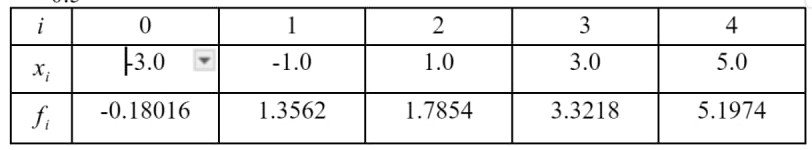
\includegraphics[width=15cm, height=4cm]{usl}
\caption{Условие}
\end{figure}
% \pagebreak

\subsection{Результаты работы}
\begin{figure}[h!]
\centering
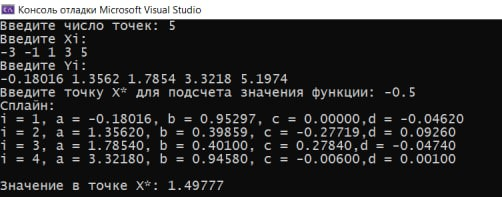
\includegraphics[width=.9\textwidth]{lab3.2}
\caption{Вывод программы в консоли}
\end{figure}

% \vfill

% \begin{figure}[h!]
% \centering
% \includegraphics[width=.9\textwidth]{lab5_taylor}
% \caption{Решение с аппроксимацией граничных условий со вторым порядком}
% \end{figure}
\pagebreak

\subsection{Исходный код}
% \lstinputlisting[language=C++]{matrix.cpp}
% \begin{lstlisting}
\lstinputlisting{include/lab3_2.cpp}
\lstinputlisting{include/tridiag.cpp}
\lstinputlisting{include/spline.h}
% \end{lstlisting}
% \lstinputlisting{matrix.cpp}
% {../../include/matrix.cpp}
% \pagebreak
% \lstinputlisting[title=\texttt{parabolic\_pde.hpp}]{../../include/partial_differential/parabolic_pde.hpp}
% \pagebreak
% 